\begin{figure}[htbp]
  \centering
  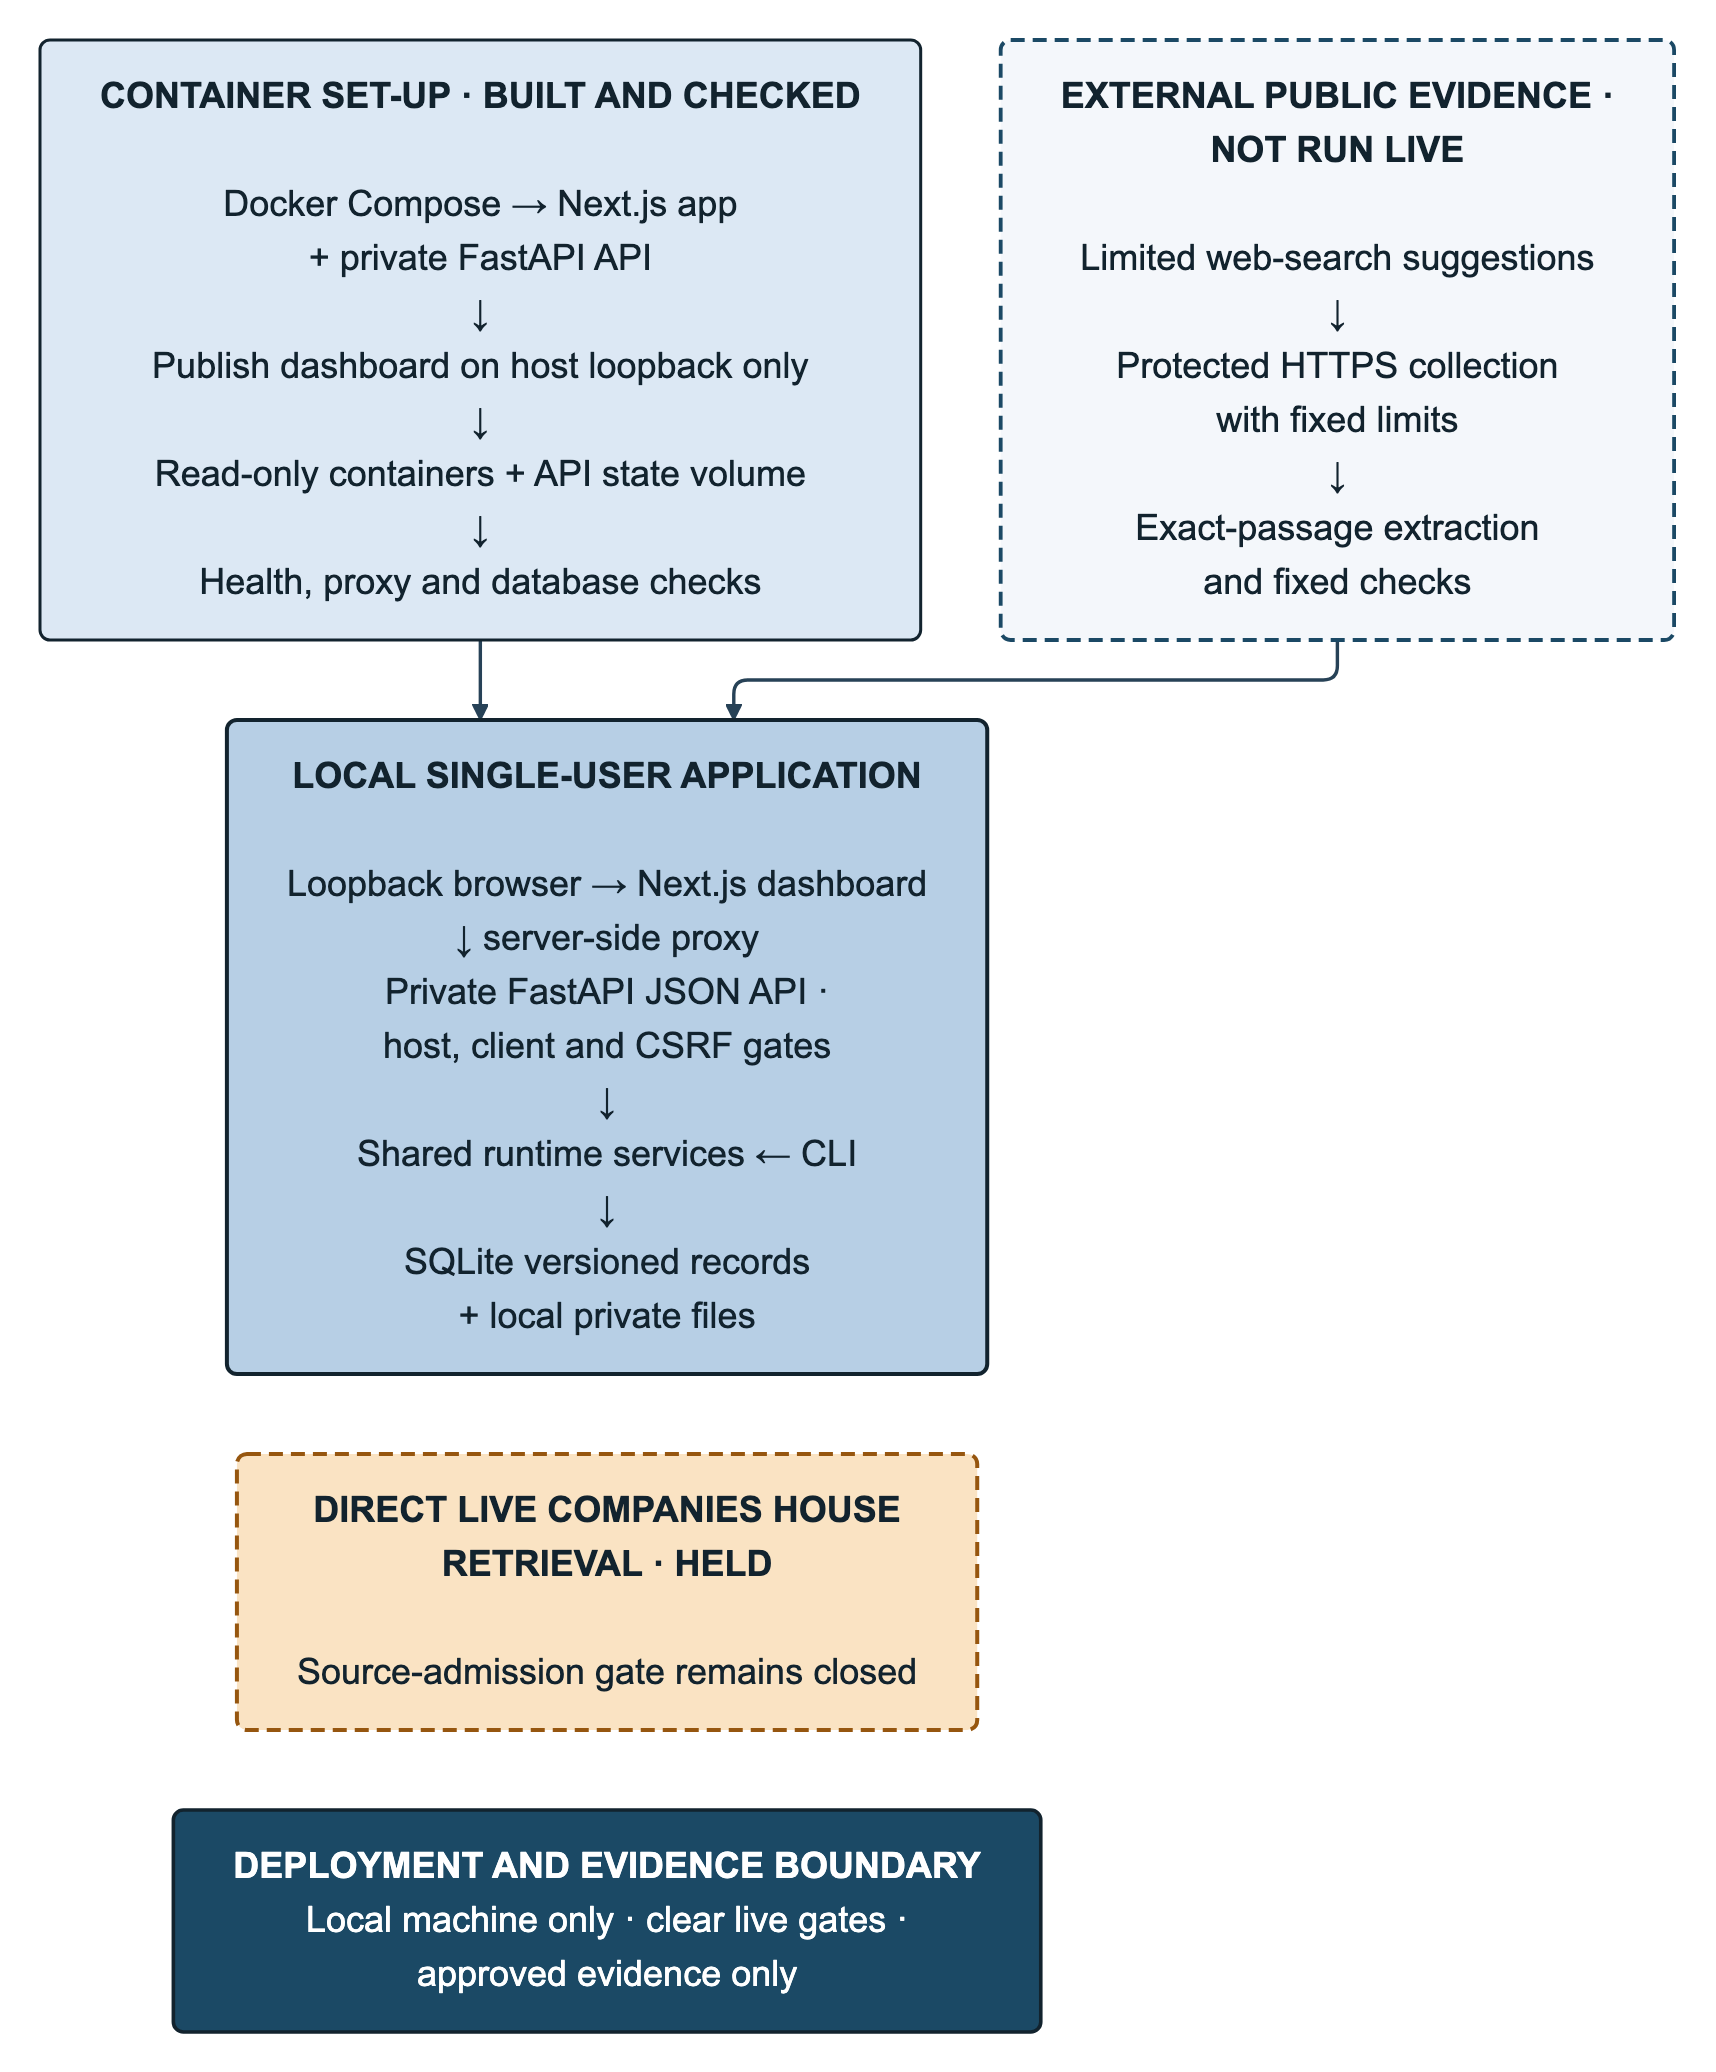
\includegraphics[width=\textwidth,height=0.42\textheight,keepaspectratio]{exhibits/sys_f1_architecture_deployment_boundary.png}
  \caption{Operator view of the local prototype: the dashboard reaches the API only through a
  private proxy, and restricted files stay on the machine. This is not a usability result.}
  \label{fig:op-local-architecture}
\end{figure}

\begin{figure}[htbp]
  \centering
  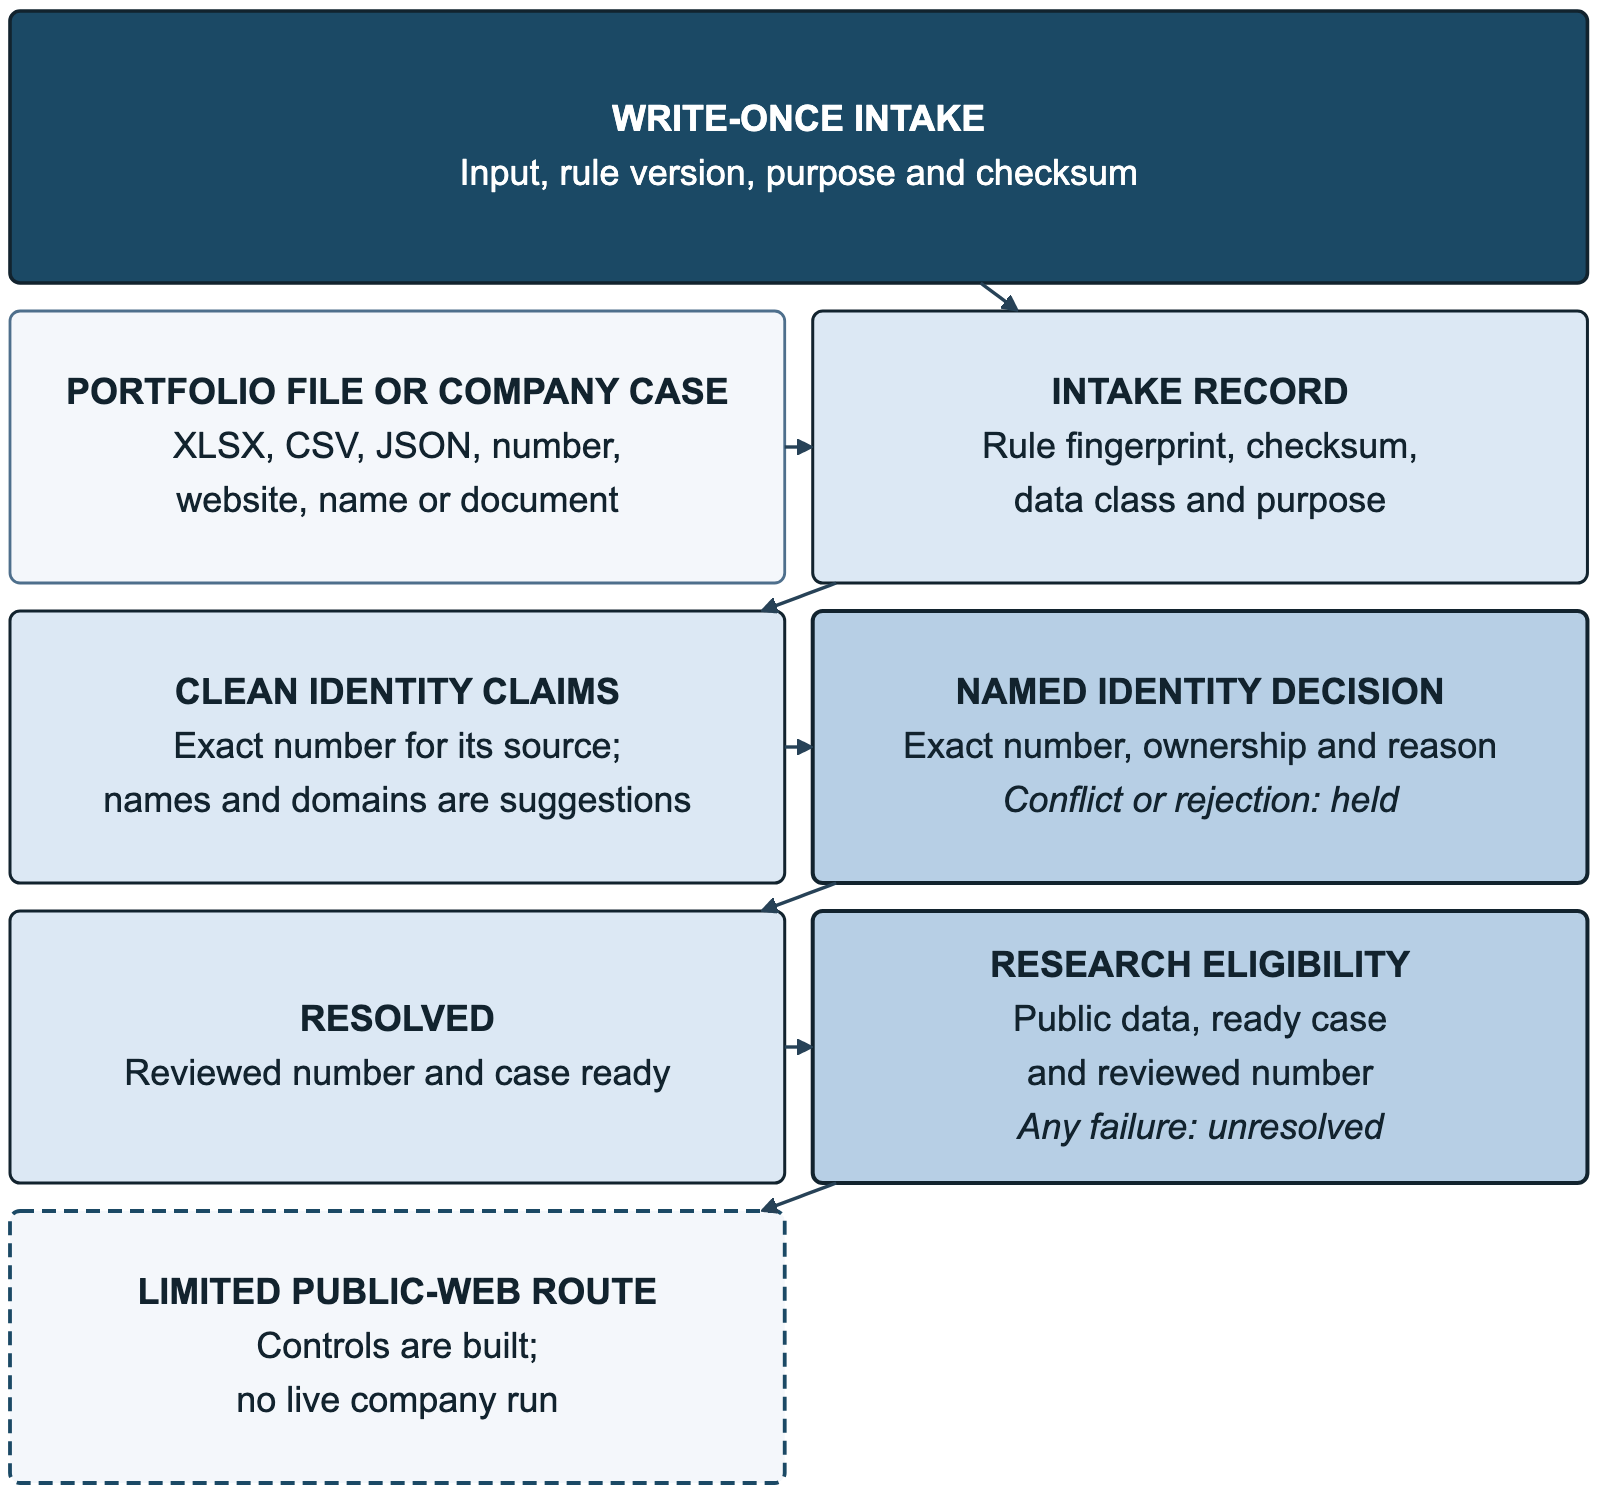
\includegraphics[width=\textwidth,height=0.42\textheight,keepaspectratio]{exhibits/sys_f3_legal_identity_decision_flow.png}
  \caption{Operator view of the implemented identity hold: a Companies House number remains a
  claim until a named person accepts it. This is not a usability result.}
  \label{fig:op-identity-hold}
\end{figure}

\begin{figure}[htbp]
  \centering
  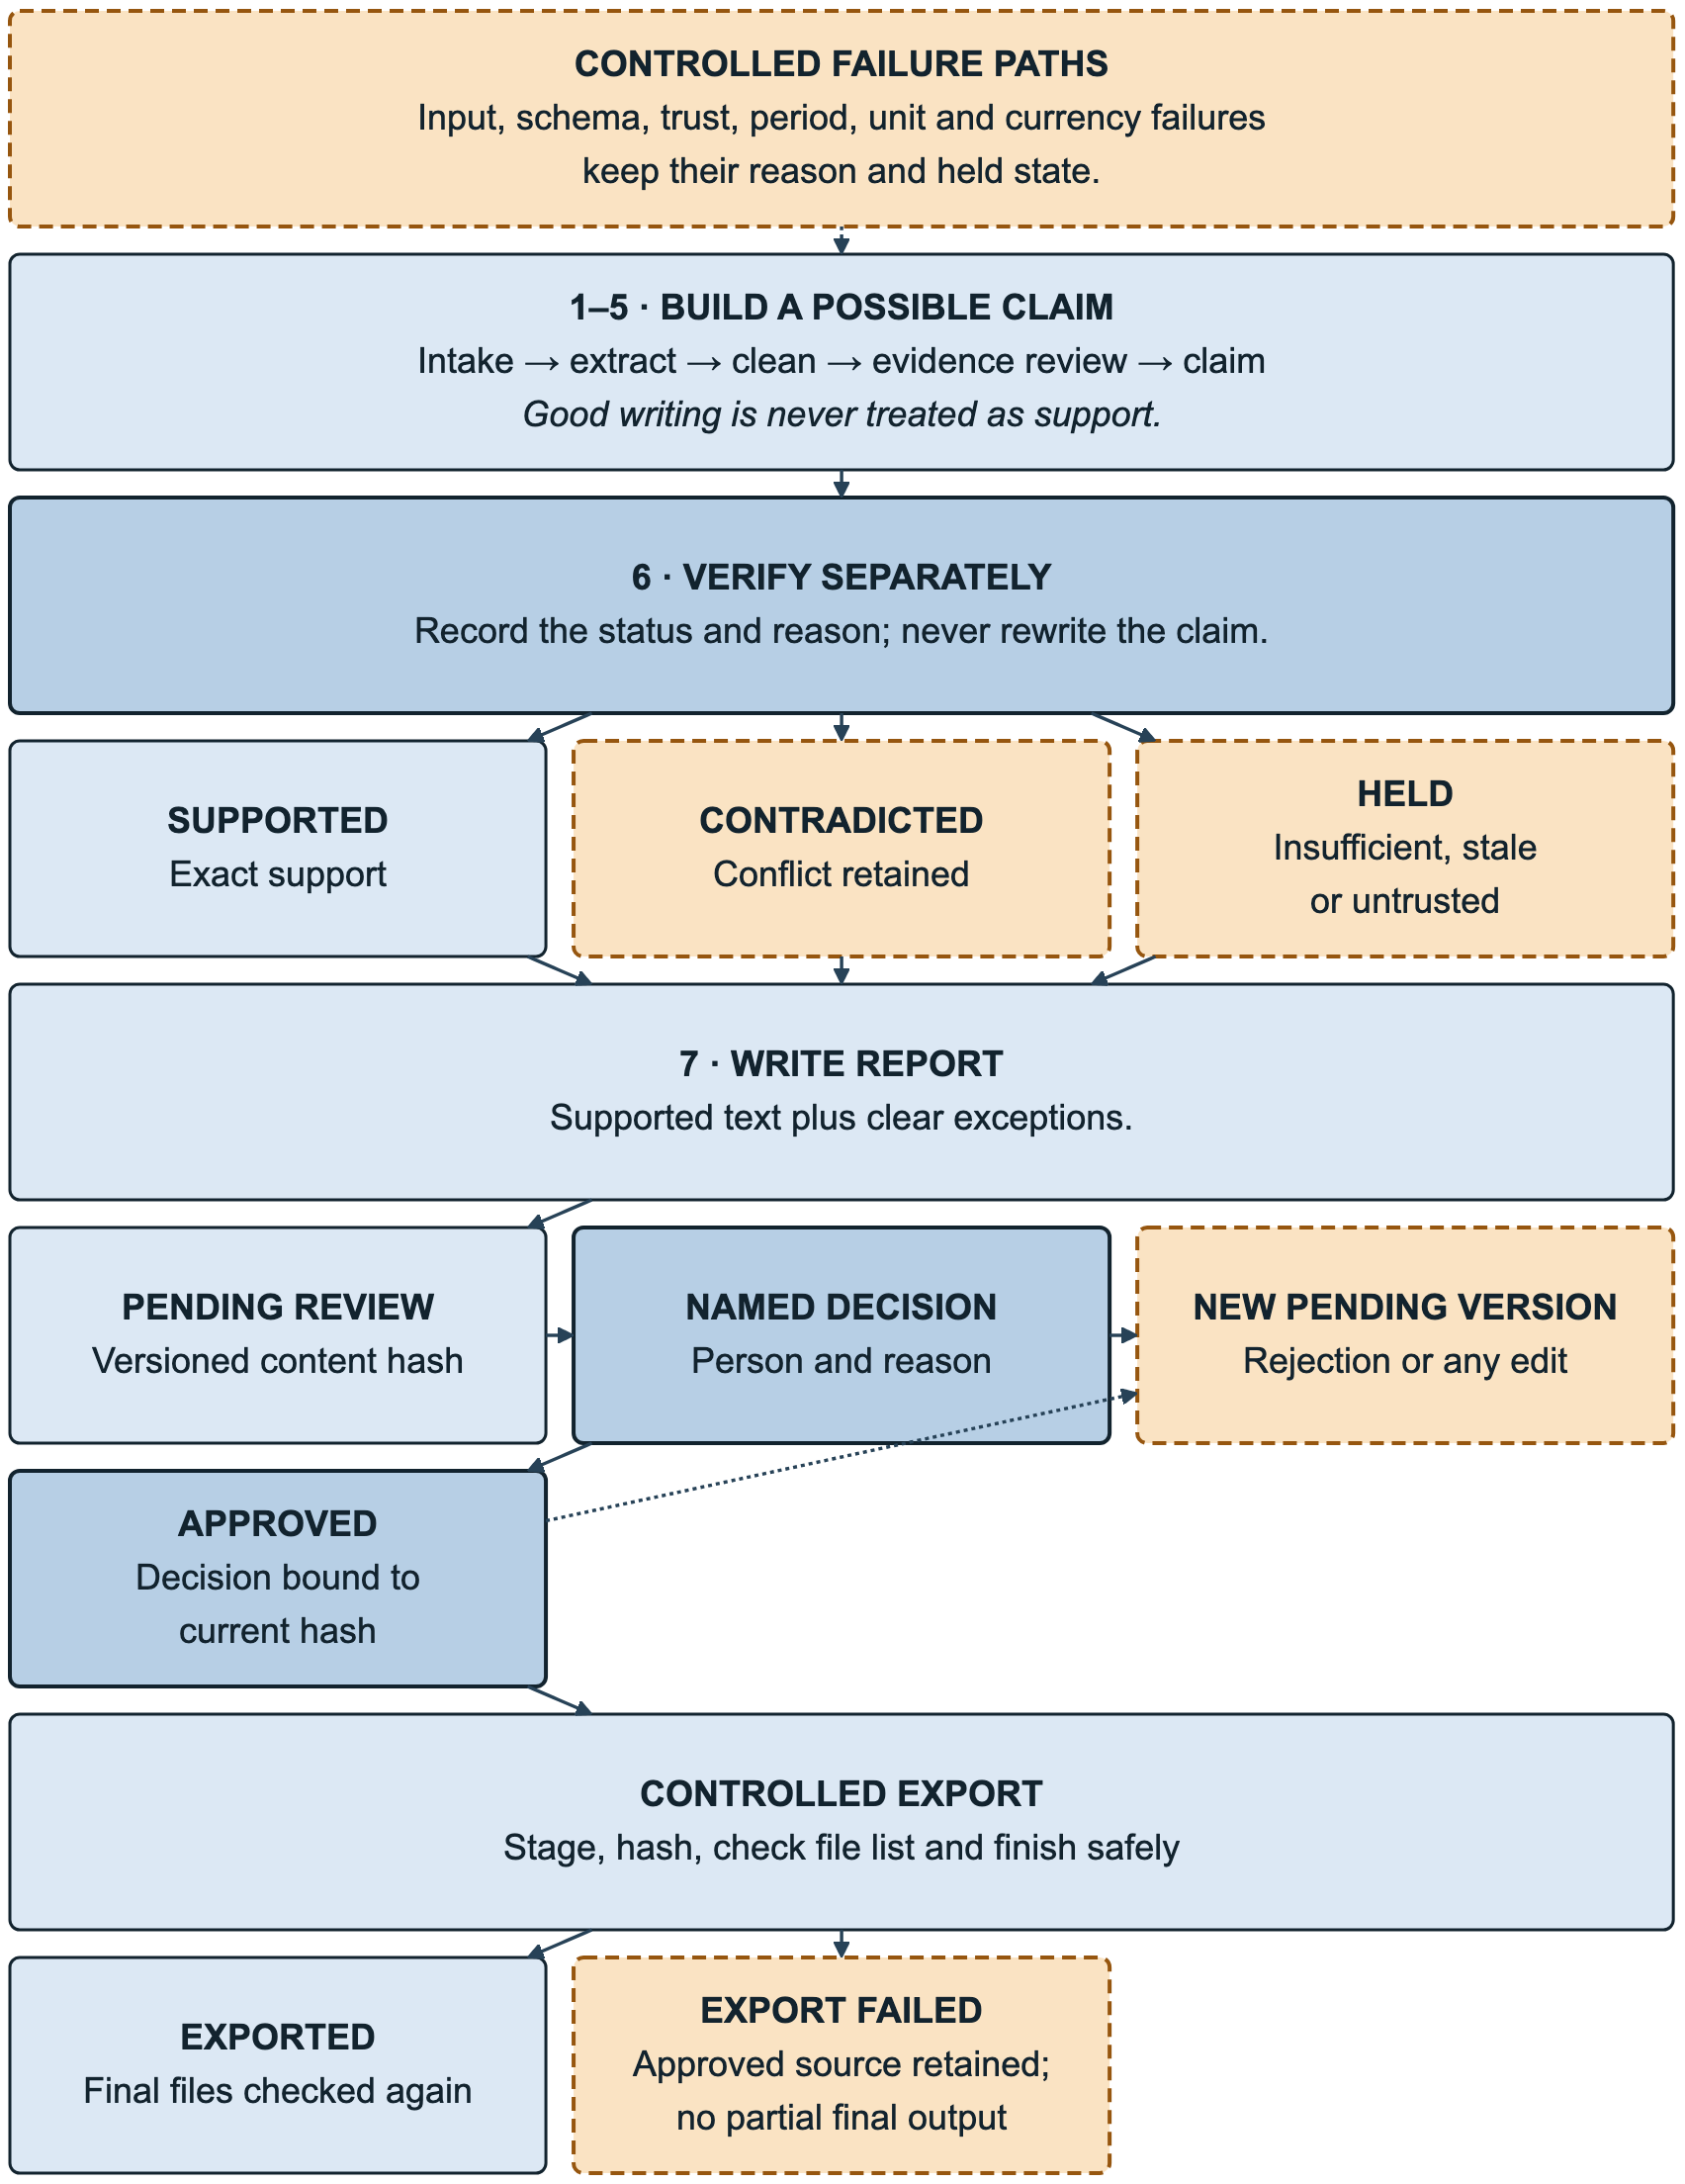
\includegraphics[width=\textwidth,height=0.42\textheight,keepaspectratio]{exhibits/sys_f4_fixed_workflow_verification_state_machine.png}
  \caption{Operator view of the implemented verification states, named approval and export lock.
  This is not a usability result.}
  \label{fig:op-verification-export}
\end{figure}

\begin{table}[htbp]
  \centering
  \scriptsize
  \setlength{\tabcolsep}{2.5pt}
  \renewcommand{\arraystretch}{1.12}
  \begin{tabularx}{\textwidth}{@{}P{0.20\textwidth}P{0.26\textwidth}P{0.22\textwidth}Y@{}}
    \toprule
    \textbf{Operator distinction} & \textbf{What is kept visible} & \textbf{Unsafe collapse} & \textbf{Implemented consequence} \\
    \midrule
    Observed zero versus blank & Jobs created $= 0$ at \texttt{submission://synthetic\#B2} & Treat a typed zero as an empty cell & Zero remains sayable; a blank does not become zero \\
    Grant conflict & \pounds100 candidate against \pounds200 at \texttt{fixture://conflict} & Average, newest-wins or larger figure & Claim withheld; disagreement retained for a named person \\
    Named approval and export lock & Actor, reason and content hash on the current version & Export after an unreviewed edit & Export stays blocked until current approval \\
    \bottomrule
  \end{tabularx}

  \caption{Implemented operator surfaces for missing-state, conflict and export lock. These are
  the local controls, not a usability study.}
  \label{tab:op-missing-conflict}
  \vspace{3pt}

  \parbox{\textwidth}{\scriptsize
    \textit{Source note:} Values from \texttt{fixtures/evaluation\_cases.json}. The table
    restates the implemented distinctions. It does not report participant behaviour.}
\end{table}
